\documentclass{proc}
\usepackage{graphicx}
\usepackage{mathtools}
\usepackage{fixltx2e}
\usepackage{algorithm}
\usepackage{algpseudocode}
\usepackage{caption}
\usepackage{url}
\usepackage{amsmath}
\usepackage{mathrsfs}

\title{
The GitHub Open Source Development Process
\author{Kevin Peterson\\
Department of Information Technology\\
Clinical Informatics Support Systems\\
Mayo Clinic\\
200 1st Street\\
Rochester, MN  55905\\
\small \texttt{peterson.kevin@mayo.edu}
}
}

\begin{document}
\maketitle

\begin{abstract}
Open Source Software (OSS) projects, or software projects with publicly available source code, are realizing ever more important roles in both personal and business computing. As such, shifts in the way in which OSS is developed could have impacts on both the quantity and the quality of OSS projects.

The development process by which these projects are produced is generally unstructured compared to commercial software, but many projects do exhibit general development patterns. GitHub, a popular OSS code hosting website, along with Git, the site's Source Code Management (SCM) tool of choice, may have the potential to fundamentally change this process by facilitating new patterns and opportunities for developers.

By analyzing a subset of GitHub repositories, this report will show how GitHub has influenced some intrinsic aspects of traditional OSS development, such as developer hierarchies and issue close velocity. We find that many of the traditional aspects of OSS development remain, such as most project development being done by a small group of core developers. Other traditional assumptions about OSS developer hierarchy, such as a large number of Issue Reporters compared to Committers, seems unsupported by the GitHub data. We conclude that GitHub represents an evolution of the OSS development process, and not necessarily a large shift.
\end{abstract}

\noindent \\\textbf{Keywords.} Git, GitHub, Open Source

\section{Introduction}
Open Source Software (OSS) has fundamentally changed how we view the Software Development Process~\cite{raymond1999cathedral}. OSS projects are not only viable, but successful and thriving. 

A case study of the Apache Server project~\cite{mockus2000case} showed that a dedicated community can produce software that rivals or exceeds commercial offerings. Furthermore, it showed that even in the unstructured context of OSS, certain structures, hierarchies, and codes of conduct emerge. Contrast the Apache Server project to a successful project on GitHub. Although the spirit and intent may be the same, the tool set is drastically different. The intent of this work is to explore how GitHub facilitates this process, and also how it may be causing it to evolve.

GitHub\footnote{https://github.com/} is a popular code hosting website that uses Git Source Code Management (SCM).\footnote{http://git-scm.com/} Along with hosting software repositories, GitHub incorporates the social aspects of development. GitHub users have community-visible profiles, and user actions can be tracked and followed by other community actions. This type of social integration of a user's identity and actions is unique to GitHub~\cite{dabbish2012social}. 

Git itself, the SCM of GitHub, lends itself to the collaborative nature of GitHub by allowing for development to take place in a more distributed manner than previously available in other SCM systems~\cite{spinellis2012git}.
Git also allows for a variety of work flows~\cite{chacon2009pro}. These work flows may be tailored to the individual needs of a project. The Linux Kernel, for example, uses a Dictator and Lieutenants Workflow~\cite{platschekfloss}, which is hierarchical in nature. Other work flows may be more distributed, or resemble more traditional centralized SCM systems. Although work flow techniques aren't explicitly addressed in this work, it is important to note that work flow change may contribute to \textit{process change}.

To better understand quantitatively the GitHub process, three hypotheses are introduced. The goal of these hypotheses is to bridge the gap between the more qualitative research of GitHub~\cite{dabbish2012social,begel2013social} and the statistical analysis of data from a random sampling of GitHub projects.

In addition, three supporting research questions are proposed. These questions will draw upon data from this work, but also reference several case studies to better represent how GitHub may be changing the way in which OSS development is conducted. These qualitative observations, paired with the more quantitative data analysis, allow for a broad description of the way that GitHub is changing the Software Engineering landscape for OSS.

\subsection{Hypotheses}
The following hypotheses are presented in an effort to better understand the GitHub development process by analyzing data from actual GitHub projects. Each hypothesis will be backed by previous research in an attempt to show concrete ways in which GitHub may be changing the OSS development process. Where possible, results from previous research on the Apache Server~\cite{mockus2000case} is compared, as this work closely aligns with Hypothesis 2 and 3.\\

\noindent \textbf{Hypothesis 1: As the number of Watchers increase, the number of Repository Forks will increase.}\\
In Open Source Software, a feeling of community belonging can be intrinsically motivating to developers~\cite{lakhani2003hackers}. This feeling of belonging can be expressed passively, as a \emph{watch}, or actively, as a \emph{fork} of a repository. 

In GitHub, a \emph{watch} is a user act of subscribing to changes in a repository. It is also referred to as a \emph{star}. A \emph{watch} allows users to receive status updates, such as when code has been committed. This is considered a \emph{passive} act, as it signifies involvement in the community, but no direct action to contribute.

A \emph{fork} is the creation of a personal copy of a repository~\cite{dabbish2012social}, from which changes may be made without impacting the original code source. A \emph{fork} is an \emph{active} action, as it signifies both involvement and intent to contribute. It should be noted, however, that it only signifies \emph{intent} -- a \emph{fork} of a repository could be made and no further actions taken.

As \emph{watches} don't necessarily signal intent to contribute, a positive direction for an OSS project is to not only increase the number of \emph{watchers}, but also the number of \emph{forks}. As both signify a general general interest in the project, it is expected that there will be some correlation between the two.\\

\noindent \textbf{Hypothesis 2: As the number Repository Forks increase, the Issue Resolution Time will decrease.}\\
In OSS, a project \emph{fork} has at times carried negative connotations, and has even been referred to as a hazzard~\cite{kogut2001open}. In the context of Git and GitHub, however, a \emph{fork} is a positive occurrence for a project, as it signifies greater project involvement. As Git allows for easy merging of \emph{forks}, code contributions in the form of defect fixes can be incorporated quickly. Because of this, it is expected that \emph{Issue Resolution Time} will decrease as the number of \emph{forks} increases.

The Apache Project noted that a rapid response to problems can be obtained because OSS is not bound to release schedules in the same way as commercial software. ``Patches'' may be released at any time, by any member of the community~\cite{mockus2000case}. ``Patches'' in the context of GitHub could be equated to \emph{Pull Requests}. A \emph{Pull Request} is an announcement by a \emph{fork} that there have been changes made that may be appropriate to add back to the main repository. The owners of the main repository may then audit these requests, and \emph{pull} some or all of them back into the main repository.

This hypothesis is, ultimately, an examination of ``Linus Law"~\cite{raymond1999cathedral} in the context of GitHub. In other words, the more exposure the code gets (in terms of forks), the easier bugs will be to find and fix.\\

\noindent \textbf{Hypothesis 3: There will be more Issue Reporters than Committers by an order of magnitude}\\
Research into the Apache Server project observed that there were far more \emph{Issue Reporters} than there were code \emph{Committers}~\cite{mockus2000case}. The Apache Server project is an excellent case study in this type of Developer Hierarchy. Apache is built around a small set of {\it Core Developers}, followed by {\it Defect Repairers} and {\it Defect Reporters}. Each level of this hierarchy brings with it an order of magnitude increase in number of participants. The 10-15 {\it Core Developers} contribute around 80\% of the new functionality, while the rest of the 400 code contributors focus primarily on bug fixes. The {\it Defect Reporters} were by far the largest group, with over 3000 individuals submitting bug reports.

Because issue reporting is of low risk to the code base, but has potentially high value, it is a perfect way for large numbers of people to contribute. It is expected that the findings of the Apache Server project research will hold true for GitHub projects as well.

\subsection{Research Questions}
To expand the analysis scope slightly, three qualitative research questions are posed. These, although backed by analyzed data where possible, are intended to show broader patterns, ideas, and motivations around the use of GitHub. Where possible, interviews~\cite{begel2013social} were conducted to explore high level concepts and motivations.\\

\noindent \textbf{Research Question 1: Are GitHub projects primarily focused around a small set of core Committers?}\\
A small core of developers contributing to a project seems to be a well entrenched pattern of OSS development~\cite{mockus2000case,mockus2002two,krishnamurthy2002cave}. At the extreme of this, a study of projects on the software hosting site Sourceforge\footnote{http://sourceforge.net} found that a large percentage of OSS development is done by lone developers~\cite{krishnamurthy2002cave}. Is a small core of developers intrinsic to OSS development, or have the social aspects of GitHub and the distributed nature of Git changed this?\\

\noindent \textbf{Research Question 2: How is GitHub changing the OSS process?}\\
The social aspects of GitHub are an important part of the development experience~\cite{dabbish2012social}. User interactions and social pressures can drive OSS development in interesting ways. Social aspects of OSS development have existed before GitHub, with mailing lists~\cite{mockus2000case}, gift giving mechanisms~\cite{bergquist2008power}, and other collaboration tools. What is GitHub doing to facilitate change in OSS development, and how does it see OSS development changing moving forward?\\

\noindent \textbf{Research Question 3: Can GitHub be used for more than code artifacts?}\\
The Object Management Group\textsuperscript{\textregistered}\footnote{http://www.omg.org} is a computer industry consortium focused on technology standards. Potential standard submission teams must go through a vetting process~\cite{kobryn1999uml} which allows industry representatives to provide feedback on the standard. Gathering and recording this feedback is a challenge, but GitHub's issue tracking system may be able to streamline the process. This just one example of how GitHub is being used for non-code artifacts. Are organizations exploring this type of work flow?

\section{Methods}
\subsection{Collection and Storage}
Data collection was done using the GitHub REST API.\footnote{http://developer.github.com/v3/} A random selection of 1000 repositories was selected, and metrics were gathered. Only repositories owned by a GitHub \textit{Organization} were considered. GitHub \textit{Organizations} are group-owned accounts,\footnote{https://github.com/blog/674-introducing-organizations} as opposed to normal individual user-owned accounts. \textit{Organization} owned repositories were chosen to increase the likelihood of analyzing high-participation projects. The selection process used for choosing the repository sample is described in Algorithm~\ref{algo:data_collection_algo}.

\begin{algorithm}[H]
\captionof{algorithm}{Data Collection Algorithm}\label{algo:data_collection_algo}
\begin{algorithmic}[1]
\While{$i < 1000$} 
\State $i \gets i + 1$
\State $word \gets \textsc{random}(word\_list)$
\State $repos \gets \textsc{github\_search}(word)$
\State $j \gets \textsc{random}(repos)$
\State $repo \gets repos_j$
\If { $\textsc{isOrgRepo}(repo)$  }
\State $\textsc{store}(repo)$
\EndIf 
\EndWhile
\end{algorithmic}
\end{algorithm}

When a random repository has been selected, the \textsc{isOrgRepo} function will filter out all non \textit{Organization} owned repositories. Next, the \textsc{store} function accepts as an input the given repository. The purpose of this function is to persist the given repository to a database for further analysis. Results were stored in a MySQL relational database management system. The database schema to store the data is described in Figure~\ref{fig:er_diagram}.

\begin{figure}
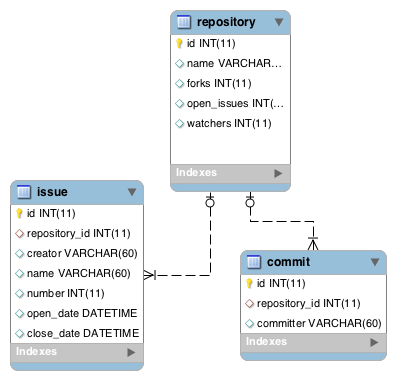
\includegraphics[height=3in,width=3in]{images/er.png}
\caption{GitHub Date Entity Relationship diagram}
\label{fig:er_diagram}
\end{figure}

Data was collected and analyzed using a Python\footnote{http://python.org/} script. Because the GitHub REST API constrains the number of API calls per hour made by a client, logic was included to pause execution when the allotment was exhausted.

Matplotlib~\cite{Hunter2007}, a 2D graphics package for Python, was used to render graphs and charts. NumPy and SciPy~\cite{scipy} were used for data analysis calculations, such as correlation coefficients.

All source code and materials used in data collection and analysis are hosted at GitHub (naturally!), and may be accessed by the following URL: \url{https://github.com/kevinpeterson/github-process-research}.

\subsection{Analysis}
As stated, the main focus of data collection was to gather metrics pertaining to GitHub \textit{Repositories}. In this context, a \textit{Repository} is defined as a set of \textit{Attributes}. An \textit{Attribute} is a metric of interest. See Section~\ref{sec:attributes} for further information on individual \textit{Attributes}. For analysis purposes, these metrics of interest are used as an Indexing Set $A^\prime$, and have labels as follows:

\[A^\prime = \{i, c, i^\prime, i^{\prime\prime}, \Delta, \omega, \epsilon\}\]

Where $i$ = {\textit{Issues}, $c$ = {\textit{Commits}, $i^\prime$ = {\textit{Closed Issues}, $i^{\prime\prime}$ = {\textit{Open Issues}, $\Delta$ = {\textit{Issue Close Time}, $\omega$ = {\textit{Issue Creators}, and $\epsilon$ = {\textit{Committers}.

All analyzed \textit{Repositories} can be thought of as the Indexed Family of \textit{Attribute} Sets, or a set of sets of \textit{Attributes}. Let the set of these sets of \textit{Attributes} be called $S$, or the \textit{Repository Sample}. We can label the \textit{Attribute} sets by arbitrary integers 0 through $|S|$, or:
\[ \{A_i\}_{i \in \{0,1,2 ... |S|\} }\]

In this way, we can reference a set of \textit{Attributes} (or, an individual \textit{Repository}), by $A_i$. 

Going further, we can also denote an individual \textit{Attribute} of a given \textit{Repository} by:
\[ \{A_{(i,\alpha)}\}_{(i,\alpha) \in A^\prime \times \{0,1,2 ... |S|\} } \]
or, $A_{i,\alpha}$. For example, $A_{10,\Delta}$ would denote the value of the \textit{Issue Close Time} ($\Delta$) of Repository \textit{10}.

To gather the metrics, the sets of all individual \textit{Attribute} across all \textit{Repositories} are processed by some aggregate function $f$. The input of this function is the union of all sets of a particular \textit{Attribute} over each \textit{Repository} in the sample. For this analysis, the aggregate functions are: \textsc{mean}, \textsc{min}, \textsc{max}, \textsc{stddev}. This analysis is applied to all repositories in the sample $S$ for which data was collected. Each attribute $\alpha$ is analyzed independently, so given:
\[ g(\alpha) =f \left( \bigcup\limits_{r = 0}^{|S|}  A_{r,\alpha} \right) \]
each individual attribute is processed via $g(\alpha)$ and will result in the output of the given aggregate function. The result of each aggregate function when applied to the entire sample set of \textit{Repositories} is shown in Table~\ref{table:summary_stats}.

\subsubsection{Attributes}
\label{sec:attributes}
The individual \textit{Attribute} names, or the elements of $A^\prime$, are described below. For detailed summary statistics of these \textit{Attributes}, see Table~\ref{table:summary_stats}.\\\\
\noindent \textbf{\textit{Issues:}}
The number of issues posted to a repository's issue tracker.\footnote{https://github.com/blog/411-github-issue-tracker}

\noindent \textbf{\textit{Commits:}}
The number of individual source code commits to a repository. It is important to note that a \textit{commit} is a single transaction that changes the code contents of a repository. Actual commit ``size'' (lines of code modified, number of files changed, for example) is not taken into account.

\noindent \textbf{\textit{Closed Issues:}}
The number of issues in a repository in a state of \textsc{closed} at the time of processing.

\noindent \textbf{\textit{Open Issues:}}
The number of issues in a repository in a state of \textsc{open} at the time of processing.

\noindent \textbf{\textit{Issue Close Time:}}
The average time (in Days) taken to close a given issue in a repository. Non-\textsc{closed} issues were not counted.\\

The average is calculated using the following method. Let $d(x)$ be a function that converts seconds to a Date, and let $s(x)$ be a function that converts a Date to seconds. Let $I$ equal the Set of \textit{Issues} in a given repository, with elements comprised of tuples $(\tau, \tau^\prime)$, where $\tau$ is \textit{Issue Open Date} and $\tau^\prime$ is \textit{Issue Close Date}. We calculate \textit{Issue Close Time} by: 

\[ \Delta = d\left( \frac{\sum_{i \in I} s\left(p_{2}(i) \right) - s\left(p_{1}(i) \right)  } {|I|} \right) \]

Where for each issue $i$ in $I$, the \textit{Issue Open Date} $s( p_{1}(i))$ is subtracted from the \textit{Issue Close Date} $s( p_{2}(i))$, where $p_{1}(i)$ and $p_{2}(i)$ denote projections of the tuple, or \textit{Issue Open Date} and \textit{Issue Close Date}, respectively. The result of this is averaged and converted into a Date via $d(x)$, resulting in the average issue close time interval $\Delta$.

\noindent \textbf{\textit{Issue Creators:}}
The number of distinct users that have opened at least one \textit{Issue}.

\noindent \textbf{\textit{Committers:}}
The number of distinct users that have summited at least one \textit{Commit}.

\section{Results}

\subsection{Summary Statistics}
\label{sec:summary_statistics}
\begin{table}[!ht]
\begin{center}
\begin{tabular}{rrrrrrr}
\hline
Variable & Mean & Min & Max & Std. Dev. \\
\hline
Issues  &  30.93  &  1  &  860  &  83.18  \\
Commits  &  249.3  &  1  &  45379  &  1700.01  \\
Closed Issues  &  26.6  &  1  &  837  &  77.56  \\
Open Issues  &  11.37  &  1  &  316  &  31.63  \\
Issue Close Time  &  26.48  &  0  &  503  &  56.54  \\
Issue Creators  &  10.61  &  1  &  128  &  22.29  \\
Committers  &  4.8  &  1  &  405  &  16.39  \\

\hline
\end{tabular}
N = 1000 Repositories
\caption{GitHub Summary Statistics}
\label{table:summary_stats}
\end{center}
\end{table}

Table~\ref{table:summary_stats} describes summary statistics of the repository variables described in Section~\ref{sec:attributes}. The most evident feature of the result is the large variance. In fact, for the set of tested variables $A$, each variable $A_j$ is observed to have a larger standard deviation than the variable mean:
\begin{equation}
\forall j \in A \colon \overline{j} < \sigma_{j}
\label{eq:variance}
\end{equation}
All measured variables demonstrated this characteristic. We will refer to this characteristic as Summary Data Assertion \ref{eq:variance}.

The sample ($N = 1000$) GitHub repositories were selected, at random, out of a total of 5.7 million~\cite{githubPress} public GitHub repositories.

\subsection{Hypotheses}
\noindent \textbf{Hypothesis 1: As the number of Watchers increase, the number of Repository Forks will increase.}\\
A correlation coefficient of 0.938794181553} was observed between the number of Watchers and Forks of a repository. This suggests that a correlation between Watchers and Forks exists.

\begin{figure}
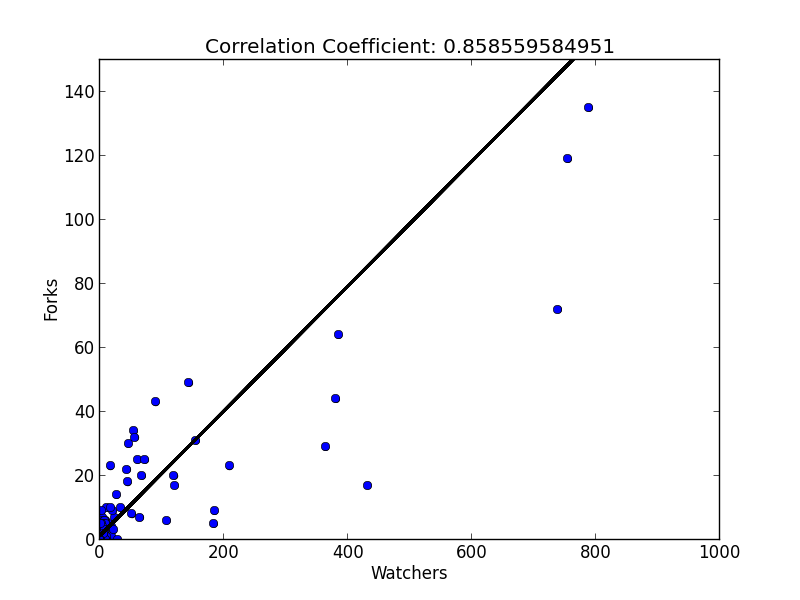
\includegraphics[height=3in,width=3in]{images/watcher_forks_scatterplot.png}
\caption{Repository watchers and forks}
\end{figure}

The data reinforces the hypothesis, as does other research in the area. Even though there are arguments that the number of Forks is the true measure of project success~\cite{baudry2012towards}, the data suggests that the two measures are related. Also, \textit{Dabbish et al.} have noted that the number of Watches can be a key for others to gauge interest in a project, and thus determine if they should participate~\cite{dabbish2013leveraging}. If the number of Watchers of a repository serves as a social cue for participation, even ``passive'' involvement with a project (Watching) could influence the ``active'' participation (Forking). This could possibly contribute to the correlation of the two variables. It is important to note, however, that we cannot conclude any causal relationship between the two variables. Concluding whether the social cue for participation is the Forks, the Watchers, or some combination, is not possible given the data and methods used.\\

\noindent \textbf{Hypothesis 2: As the number Repository Forks increase, the Issue Resolution Time will decrease.}\\
No significant correlation was found between the number of repository forks and issue resolution time. It is important to note, however, that issue resolution time is not necessarily related to software product quality in the context of GitHub. We can assert that for several reasons. \textit{First}, GitHub issues are not necessarily product defects. Issues may be feature requests, comments, or general support questions. \textit{Second}, GitHub projects may have primary issue tracking services elsewhere, while using the GitHub issues as secondary services or not at all. \textit{Third}, Pham \textit{et al.} explore an emerging ``testing culture'' in GitHub. This, among other things, suggests that GitHub may be facilitating testing by making it more \emph{triable} by lowering entry barriers, and makng the process as a whole more \emph{observable}. This aspect is something which could have sizable impacts on software quality but wouldn't necessarily be reflected in this metric~\cite{phamcreating}.

\begin{figure}
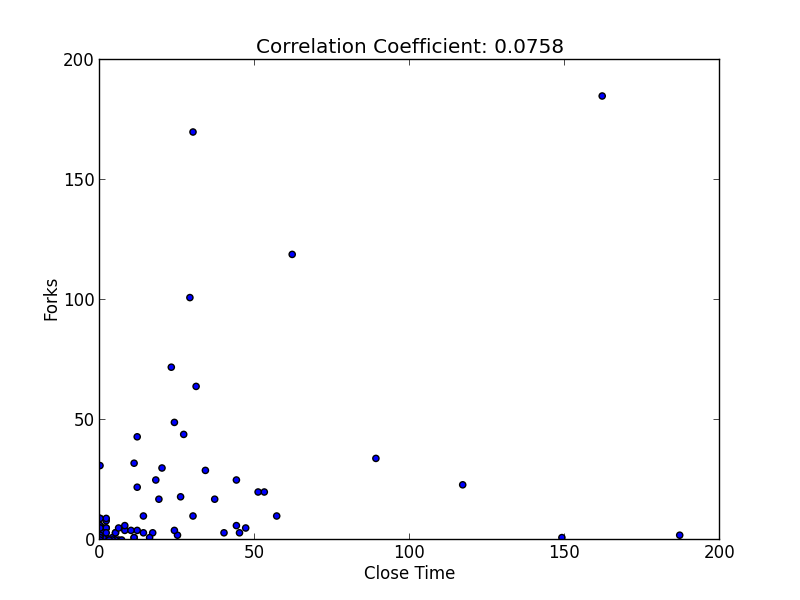
\includegraphics[height=3in,width=3in]{images/issue_close_time_forks_scatterplot.png}
\caption{Repository issue close time and number of forks}
\label{fig:issue_close_time_forks_scatterplot}
\end{figure}

It is possible that other factors, such as issue prioritization, may have a greater impact on issue resolution time. Research does support a relationship~\cite{mockus2002two} between the stated priority and fix interval. As the GitHub issue tracker can only support prioritization by free-text \textit{tags} placed on issues, it is not feasible to programmatically gather issue priority metrics.\\

\noindent \textbf{Hypothesis 3: There will be more Issue Reporters than Committers by an order of magnitude.}\\
Data does not support an exponentially increasing number of distinct Issue Reporters as compared to distinct Committers. 
As shown in Figure~\ref{fig:issue_reporters_committers_scatterplot}, the slope of the relationship between the two variables is less than one. This does not seem to completely align with findings in the Apache Server project~\cite{mockus2000case}. 

\begin{figure}
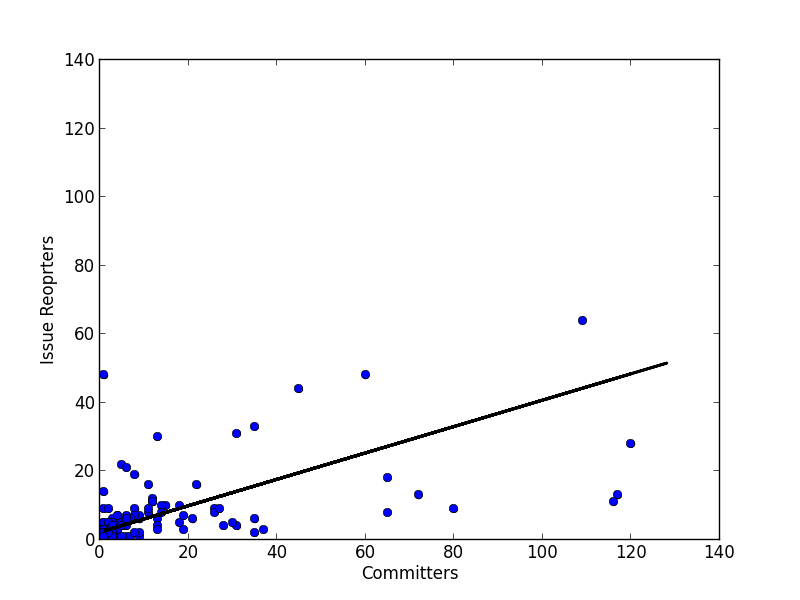
\includegraphics[height=3in,width=3in]{images/issue_reporters_committers_scatterplot.png}
\caption{Repository issue reporters and committers}
\label{fig:issue_reporters_committers_scatterplot}
\end{figure}

Figure~\ref{fig:issue_reporters_committers_scatterplot}, does however suggest, however, that that the two variables are related. The hypothesis implies that there will be a correlation between the two variables -- which is demonstrated by a reasonably strong correlation coefficient of 0.8299}\unskip. More investigation would be necessary to further examine this finding.\\

\subsection{Research Questions}
\noindent \textbf{Research Question 1: Are GitHub projects primarily focused around a small set of core Committers?}\\
The data in Figure~\ref{fig:committers_percentage_pie_chart} represents commit percentage breakdown, or an analysis of developer \textit{Contribution} percentages to a repository. The intent of this measurement is to show how the number of repository commits are distributed among it's committers. The slices represent the distribution of committers that have committed a given percentage of commits (or a \textit{Contribution} percentage, as labeled in the figure) to a project. For example, a small percentage of developers have contributed $95-100\%$ of the commits to a repository, so this is represented as a small slice in the figure. Contrast that to developers that have committed $0-5\%$ of the commits to a repository. This type of contribution is common, and represented as a larger slice. The \textit{Contribution} percentages are calculated by:

\begin{equation}
P = \left\{ \frac{ C_u } { |\mathscr{C}| } \times 100 \Big| u \in U \right\}
\label{eq:commit_percentage}
\end{equation}

Where $U$ is the Set of \textit{Committers} to a given \textit{Repository}, $\mathscr{C}$ is the set of all \textit{Commits} to a \textit{Repository}, and $C_u$ denotes sets of \textit{Commits} by an individual \textit{Committers} to a \textit{Repository}, or:
 \[ \{ C_u \}_{u \in U} \]

Each \textit{Committer}, then, will produce a subset of all \textit{Commits} to a a \textit{Repository}, or $C_u \subset \mathscr{C}$. 

\begin{figure}
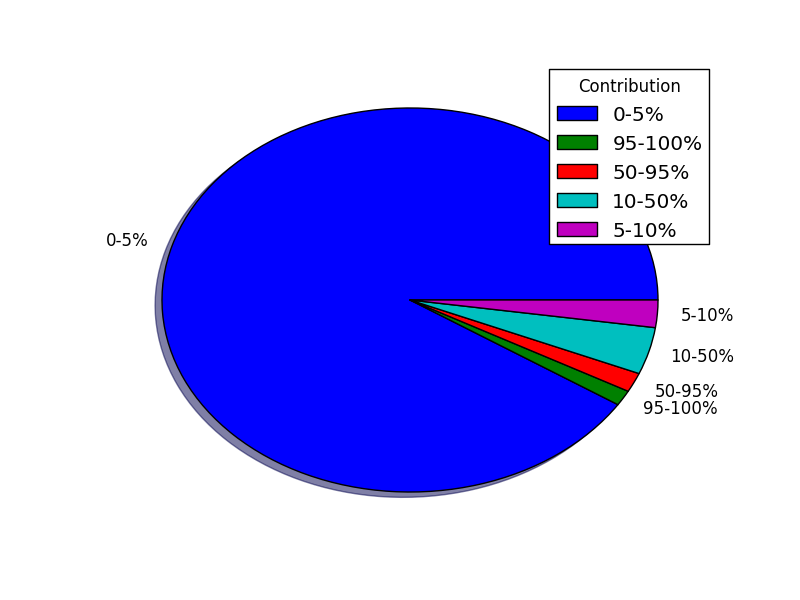
\includegraphics[height=3in,width=3in]{images/committers_percentage_pie_chart.png}
\caption{Distribution of individual committer commit percentage of a repository}
\label{fig:committers_percentage_pie_chart}
\end{figure}

To find the percentages, or set $P$ of Equation~\ref{eq:commit_percentage}, the commits by each user $C_u$ are divided by the total number of commits $|\mathscr{C}|$, yielding the set of contribution percentages $P$ for the repository. Elements of $P$ are then assigned to ranges $0-5\%$, $5-10\%$, $10-50\%$, $50-95\%$, and $95-100\%$ (with shared values inclusive to the larger range). The distribution of this range assignment is plotted on Figure~\ref{fig:committers_percentage_pie_chart}.

Most notably, the data shows that a large percentage of developers committed small amounts ($0-5\%$) of the total number of repository commits. This means that a small core are not entirely monopolizing the commits, but rather opportunity exists for users to contribute, even if in small ways. Instances of developer monopolization of commits to a repository (for example, where a developer contributes $95-100\%$ of the total commits), are shown to be small.

\begin{figure}
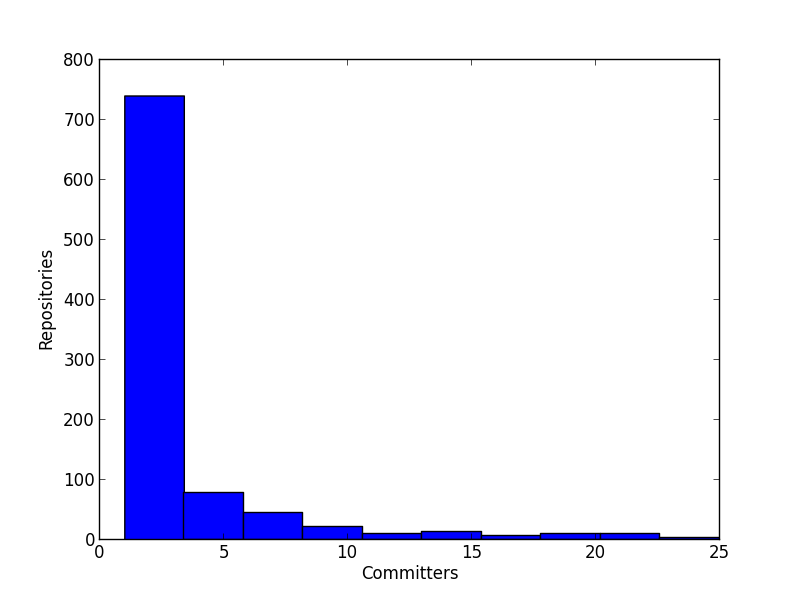
\includegraphics[height=3in,width=3in]{images/committers_histogram.png}
\caption{Count of individual committers per repository}
\label{fig:committers_histogram}
\end{figure}

When looking strictly at the number of committers to a repository, however, the notion of a small set of core committers is strongly supported, as the vast majority of repositories have fewer than 10 committers (Figure~\ref{fig:committers_histogram}).\\

\noindent \textbf{Research Question 2: How is GitHub changing the OSS process?}\\
Thung \textit{et al.} showed that the social coding aspects of GitHub -- specifically the developer-to-developer connectivity -- enabled high collaboration rates~\cite{thung2013network}. In fact, the developer connectivity was shown to be higher than SourceForge and even Facebook. In a recent interview with GitHub staff, the social aspects of GitHub were referred to as ``unique and powerful~\cite{begel2013social},'' which seems to suggest that this is a strong underlying product goal.

Ye also observed that the contribution environment, or ``society,'' is important in providing a framework for developer trust building:
\begin{quote}
Only in a society where technical supremacy is highly appreciated can developers acquire good reputations among their peers by displaying their skills through free distribution, and often wider acceptance, of their systems.The good reputation attracts attention, trust, and cooperation from others and lays the foundation for advancing the original developers agenda and the establishment and development of OSS communities.~\cite{ye2003toward}
\end{quote}

With this process change can also come cause for concern. The move to Git from a centralized version control system (such as SVN or CVS) is not without its challenges. Differences in philosophy and nomenclature may place added strain on developers~\cite{bird2009promises}. Also, it is not to be assumed that process change is always welcome~\cite{de2009software}, even if it is an improvement. Developers and organizations have existing processes, SCM tools, and workflow patterns -- which all change at a cost.

Despite the potential migration cost, the National Center for Biomedical Ontology,\footnote{https://github.com/ncbo} the National Cancer Informatics Program,\footnote{https://github.com/ncip} NASA,\footnote{https://github.com/nasa} and the WhiteHouse\footnote{https://github.com/WhiteHouse} are just some organizations that have moved all or portions of development to GitHub. As these and other organizations consider the move to GitHub, the distributed and ``social'' aspects of the OSS process will continue to evolve.

According to GitHub Staff member John Britton, lowering the barrier to participation is an important cultural shift:
\begin{quote}
GitHub moved the open source community away from a permission culture. Prior to GitHub, contributing to an open source project was very difficult and often involved asking permission. By allowing people to fork a repository and make changes without asking for permission, GitHub has made contributing to someone else's project much easier than it has ever been. By submitting a Pull Request with suggested changes, project maintainers and contributors have a place to discuss changes to code that is already written and to refine it.~\cite{github_interview}
\end{quote}

Spending large amounts of time and resources to participate is a detriment to knowledge-sharing in general, not just OSS development~\cite{ardichvili2003motivation}. Because of this, we conclude that this permissive culture of knowledge-sharing that GitHub fosters represents an important change in the OSS process.\\

\noindent \textbf{Research Question 3: Can GitHub be used for more than code artifacts?}\\
The OMG\textsuperscript{\textregistered} standardization process is a process by which products strive to produce an interoperability standard by way of an industry standards consortium~\cite{omgTechProcess}.
The standardization process itself aims to, at its conclusion, produce a set of model artifacts containing sufficient detail such that when interpreted and implemented, produce interoperable software.
At a conceptual level, this can be thought of as a software requirements engineering process as much as a standardization process. If so, of the five main tasks of requirements engineering, Elicitation, Analysis and Negotiation, Documentation, Validation, and Management,~\cite{sommerville1998requirements} we can show that GitHub is an appropriate forum for many of them.

As a case study, the CTS2 OMG\textsuperscript{\textregistered} Specification~\cite{cts2} used a GitHub issue tracker\footnote{https://github.com/cts2/cts2-specification/issues} to track specification changes. Elicitation, Analysis and Negotiation were natural fits for the issue tracker. This was chosen in part because the barrier to participation was very small (only a GitHub account was needed), and the issue tracker itself allowed for dialogs in the form of comments. Because customer involvement is critical to these activities~\cite{paetsch2003requirements}, ease of contribution was a main concern. OMG\textsuperscript{\textregistered} has a predescribed format for requirements Documentation, but using the GitHub issue API,\footnote{http://developer.github.com/v3/issues/} much of this documentation can be automated.
Validation and Management are areas of requirements engineering that GitHub has interesting solutions for. First, in order to track (or validate) changes to the specification, when the actual specification is modified, the commit that modified it can be traced to a named issue by simply putting the issue number in the commit log. This level of traceability is powerful, as it allows every change to the specification artifacts to be tracked consistently to an open issue. As the normal OMG\textsuperscript{\textregistered} process proceeds, requirements can be managed through ``tagging'' the issues. By allowing issues to be grouped by arbitrary tags, users are more free to adapt their own work flow. For instance, when community voting on issues needed to be done for CTS2, a simple ``ready for vote'' tag signified to the voting board exactly what was under consideration

As mentioned, the CTS2 specification made heavy use of the GitHub issue tracker, as well as another OMG\textsuperscript{\textregistered} specification, ServD.\footnote{https://github.com/servd/servd-specification} For open source specifications, or requirements engineering activities, GitHub has shown to be a viable platform. 

\section{Conclusion}
The analysis suggests an \textit{evolution} in process, but not necessarily a large shift. We classify this as an \textit{evolution} because although many of the traditional aspects of the OSS development process remain, there are notable differences. For example, a small subset of core developers, a traditional aspect of OSS development~\cite{mockus2000case,mockus2002two,krishnamurthy2002cave}, seems supported by both the summary data in Figure~\ref{eq:variance}, and the distribution of committers per repository in Figure~\ref{fig:committers_histogram}. Figure~\ref{fig:committers_percentage_pie_chart} shows a significant number of participators, albeit with small contribution amounts, in many repositories. This may indicate a lowered entry barrier for participation, and is consistent with the conclusions reached in Research Questions 1 and 2.

The data does not, however, reflect some other traditional aspects of OSS development. Notably, it was observed that data gathered for Hypothesis 2 and Hypothesis 3 seemed contrary to what the Apache Server report concluded~\cite{mockus2000case}. A possible explanation is the amount of variability in the data collected. Summary Data Assertion~\ref{eq:variance} (Section~\ref{sec:summary_statistics}), which is derived from the summary data shown in Table~\ref{table:summary_stats}, suggests large amounts of variety in the observed variables. This may suggest a wide range of repository purposes, or specifically, that not all repositories on GitHub are intended to be consumable software artifacts for users, or ``customers.'' A large number of repositories may not be intended for customer consumption, but merely as example code, experimentation, or exercises. Given this, and specific reasons outlined in the hypotheses themselves, we cannot state any definitive conclusions regarding these two hypotheses. More research into categorizing GitHub repositories is needed.

The most notable \textit{difference} in OSS process driven by GitHub, considering both the quantitative and qualitative analysis, is the lowered barrier to participation. Qualitative analysis conducted in Research Question 2 suggests a cultural shift~\cite{begel2013social,github_interview} in the participation process. The data also supports high levels of participation, especially Figure~\ref{fig:committers_percentage_pie_chart}, which shows that many repositories have large numbers of developers committing small amounts of code. This, we conclude, represents an important \textit{evolution} in the OSS development process.

\section{Acknowledgments}
We thank Gilberto Fragoso, Ph.D. (NIH/NCI), Paul Alexander (NCBO), John Britton (GitHub), and all of the GitHub Staff for interviews, insights and ideas, Harold Solbrig, Craig Stancl, and Dick Hedger for guidance, and Rick Kiefer for his review.

\bibliographystyle{plain}
\bibliography{bibliography}

\input{interview}
\clearpage

\section*{Appendix B: Interview Transcript}
Email interview with John Britton, Education Liaison, GitHub, April 17, 2013.

\subsection*{Q: How is GitHub changing the way Open Source Software (OSS) is being developed today?}
GitHub moved the open source community away from a permission culture. Prior to GitHub, contributing to an open source project was very difficult and often involved asking permission. By allowing people to fork a repository and make changes without asking for permission, GitHub has made contributing to someone else's project much easier than it has ever been. By submitting a Pull Request with suggested changes, project maintainers and contributors have a place to discuss changes to code that is already written and to refine it.

\subsection*{Q: Many new Software Developers will be starting their education/training already having experience with GitHub. How, in your opinion, will Software Engineering as a discipline (and how it is taught) change to accommodate the ideas popularized by GitHub?}

Software Engineering is moving more towards the development models seen in industry. It's much more useful for students to learn how to use the tools that they will see in industry than it is to learn how to use learning management systems and the like. I encourage teachers to assign project work in teams so that students gain experience working together and navigating the issues that arrive in a collaborative environment. While it's far from standard practice, I'm seeing more and more teachers encouraging and even requiring the use of version control, code review, and automated testing. Most of these tools have been standard in industry for quite a while, but only recently have they made their way into the classroom thanks to services like GitHub lowering the learning curve substantially.

\subsection*{Q: There are many non-code artifacts being hosted on GitHub, for example, Object Management Group Specifications, Laws and Statutes, books... etc. Do you see GitHub participation expanding in the non-code areas?}
Most definitely. There are many examples of non-code artifacts hosted on GitHub:

\begin{itemize}
\item German law\footnote{https://github.com/bundestag/gesetze}
\item Images\footnote{https://github.com/blog/817-behold-image-view-modes}
\item 3d models\footnote{https://github.com/blog/1465-stl-file-viewing}
\item Research papers\footnote{https://github.com/karthikram/smb\_git}
\end{itemize}

That's just a small sample of some interesting things on GitHub, we're seeing new uses all the time.

\end{document}